





\section{Frequency analysis}
\label{sec:analysis}
\subsection{Car engine}

\begin{figure}
	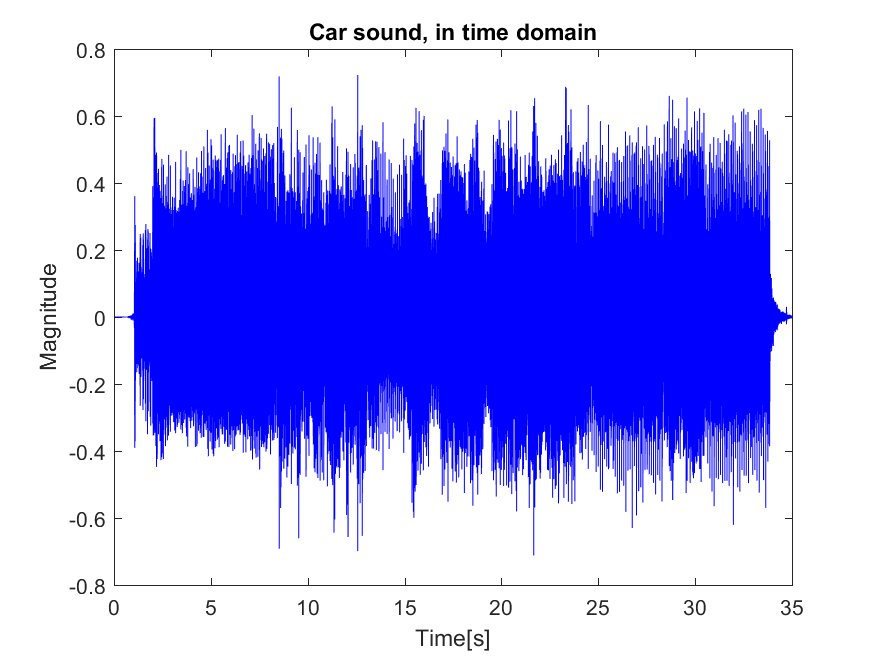
\includegraphics[width=\textwidth]{code/Car_figure1.png}
	\caption{kage}
	\label{fig:Car_figure1:1}
\end{figure}

\subsubsection{DFT}
\begin{figure}
	\centering
	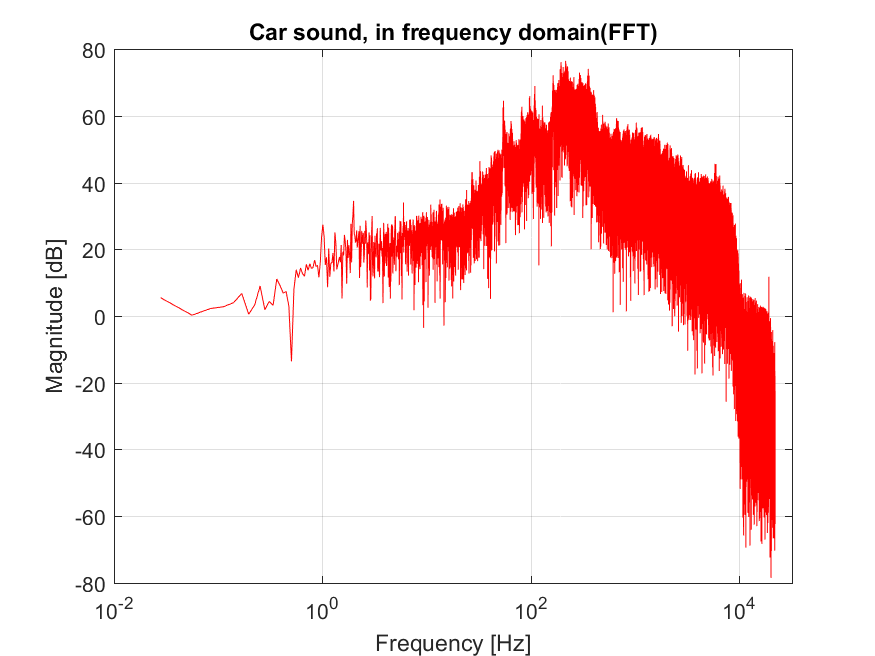
\includegraphics[width=\textwidth]{code/Car_figure2.png}
	\caption{}
	\label{fig:Car_figure2:2}
\end{figure}




\subsubsection{Analysis}



\subsubsection{Conclusion}

\subsection{Noise from a windmill}
\subsubsection{DFT}

\subsubsection{Analysis}

\subsubsection{Conclusion}

\subsection{EKG}
\subsubsection{DFT}

\subsubsection{Analysis}

\subsubsection{Conclusion}

\subsection{Breaking wine glass}
\subsubsection{DFT}

\subsubsection{Analysis}

\subsubsection{Conclusion}

\subsection{Music}
\subsubsection{DFT}

\subsubsection{Analysis}

\paragraph{Genre 1}

\paragraph{Genre 2}

\paragraph{Genre 3}

\paragraph{Genre 4}

\subsubsection{Conclusion}

\section{Further analysis of signals}
\label{sec:analysisOfSignals}
Eksperimenter med udglatning, zero-padding og windowing 

\section{Energy} 
\Cref{tab:Energy} shows the energies in signals before and after the Fourier transform. It clearly shows that there is no loss of energy between the original signal and a Fourier transform, but when smoothing and windowing is applied there is a potential loss of energy.
While zero padding does not add or remove any energy from the signal.
\begin{table}[]
	\centering
	\begin{tabularx}{\textwidth}{p{2cm} | X X X X X}
		& \rotatebox{90}{\textbf{Time Domain $\times\num{e4}$}}   & \rotatebox{90}{\textbf{Frequency Domain $\times\num{e4}$}} & \rotatebox{90}{\textbf{Smooth $\times\num{e3}$}}     & \rotatebox{90}{\textbf{Zero Padding $\times\num{e4}$}}  & \rotatebox{90}{\textbf{Windowing $\times\num{e4}$}} \\
		\hline
		Windmill	& \num{4,14}	& \num{4,14}	& \num{0,521} & \num{4,14} & \num{1,79} \\

		Car Engine  & \num{3,07}	& \num{3,07}	& \num{0,686}  &	\num{3,07}  & \num{1,34}  \\

		Cheerleader & \num{13,4}	& \num{13,4}	& \num{1,29}	& \num{13,4}	& \num{7,39}  \\

		Roundtable Rival & \num{29,8}	& \num{29,8}	& \num{1,70}	& \num{29,8}	& \num{12,8}5  \\

		Micheal Jackson \newline Billie Jean & \num{16,3}	& \num{16,3}	& \num{1,73}	& \num{16,3}	& \num{6,86} \\

		Violin \newline Let It Go & \num{2,24}	& \num{2,24}	& \num{0,896}	& \num{2,24}	& \num{1,09}  \\

		Krystalglas knuses & \num{0,0115}	& \num{0,0115}	& \num{0,155}	& \num{0,0115}	& \num{0,000265} \\

		EKG & \num{2,05}	& \num{2,05}	& \num{0,626}	& \num{2,05}	& \num{0,729}
	\end{tabularx}
	
	\caption{Energy of the different signals shown in \si{\joule}.}
	\label{tab:Energy}
\end{table}

\section{Discussion}

Skalering --> Vi kan ikke bruge frekvenser højere end nyquits frekvens ?
Korrekte frekvensbins?

\section{Conclusion}